\documentclass[article]{report} % Type of document

\usepackage[utf8]{inputenc}    		 	% Encoding
\usepackage[english]{babel}			% Language
\usepackage{geometry}           			% Page margin
\usepackage{graphicx}           			% For images
\usepackage{newcent}            			% Font
\usepackage{color}              			% Colors
\usepackage{listings}           			% Lists
\usepackage[footnote, nolist]{acronym}	% Acronyms
\usepackage[absolute, overlay]{textpos}	% Text positioning

\usepackage{fancyhdr}          			 % We might have a need for them
\usepackage{float}
\usepackage{tabularx}

\usepackage{latexsym}
\usepackage{pdfpages}
\usepackage{tikz}
\usepackage{ifthen}
\usepackage{wrapfig}
\usepackage{textcomp}
\usepackage{multicol}

\setlength{\columnsep}{1cm}
\setlength{\TPHorizModule}{\paperwidth}	% Used for textblock
\setlength{\TPVertModule}{\paperheight}	% Used for textblock

\title {Book of specifications}
\parskip = 0.25cm              % Summary options (spaces between lines)

% Margin
\geometry{tmargin=2.5cm, bmargin=1.5cm, lmargin=2.5cm, rmargin=2cm}

\definecolor{blue}{rgb}{0.13,0.29,0.46}
\definecolor{red}{rgb}{1,0,0}
\definecolor{couleur_titre}{rgb}{0.20, 0.45, 0.80}
\definecolor{couleur_nom}{rgb}{0.11, 0.6, 0.18}

\renewcommand{\labelitemi}{$\bullet$}
\renewcommand{\contentsname}{Table of contents}

% Title at the top of the page
\pagestyle{fancyplain} \chead{}\lhead{\textit{Team Dedalus}} \rhead{\textcolor{couleur_titre}{\emph{\textit{Project: Islands}}}}

\title {Book of specifications}
\author {Romain\and Renaud\and Aenora\and Erwan}
\date {}

%
% Document
%
\begin{acronym}
	\acro{OO}{Oriented-Object}
	\acro{RTS}{Real Time Strategy}
	\acro{FPS}{First Person Shooter}
	\acro{Mogre}{Managed Object-Oriented Graphics Rendering Engine}
	\acro{API}{Application Progamming Interface}
	\acro{GUI}{Graphical User Interface}
	\acro{MyGUI}{Multilayer and overlappable GUI System}
	\acro{IDE}{Integrated Developement Environment}
	\acro{AI}{Artificial Intelligence}
	\acro{NPC}{Non Player Character}
	\acro{UML}{Unified Modeling Language}
	\acro{PHP}{PHP : Hypertext Preprocessor}
	\acro{ORM}{Object-Relational Mapping}
	\acro{MVC}{Model View Controller}
	\acro{OGRE}{Object-Oriented Graphics Rendering Engine}
\end{acronym}
\begin{document}
		\thispagestyle{empty}
  			\begin{titlepage} 
						\vspace*{1cm} 
  					\begin{center} 
  							{\huge{\textsc{1st Oral} \\ ~ \\{\large From}\\ ~\\ Team \\  ~ \\ }}
	  						\includegraphics[width = 14cm]{Images/Dedalus.png}
							\\ ~ \\ ~ \\ ~ \\ ~ \\ ~ \\ ~ \\ ~ \\ ~ \\ ~ \\ ~ \\ ~ \\ ~ \\ ~ \\ ~ 
						\end{center}
  					\hfill {\large Romain \textsc{Biessy}}
  					\hfill {\large Renaud \textsc{Gaubert}}
  					\hfill {\large Aenora \textsc{Tye}}
  					\hfill {\large Erwan  \textsc{Vasseure}}
  			\end{titlepage} 

  	\tableofcontents
  			\pagenumbering{arabic}
  			\newpage
				\chapter{\textcolor{blue}{Introduction}}


					 We also decided that we would make a 3D game at the first person. Also we thought about a mix between \ac{RTS} and \ac{FPS}. \\ 						Creating a game has never been an easy task but, the game we imagine could be described as ambitious. Nevertheless, our teamwork should not be underestimate.\\
					We will code this game with the help of \ac{Mogre} which is a 3D engine using C\#.  
 								
								
  			\chapter{\textcolor{blue}{Gameplay}}
						\section{RTS \& FPS \& minecraft-like}
								We decided that our game would be a mix of an \ac{RTS} and an \ac{FPS} on a minecraft-like terrain. What does that mean ? Basically, it means that you will be a following a character at first person. Besides Minecraft-like terrain means that he will be walking on cubes :\\ 
							\begin{figure}[h]
								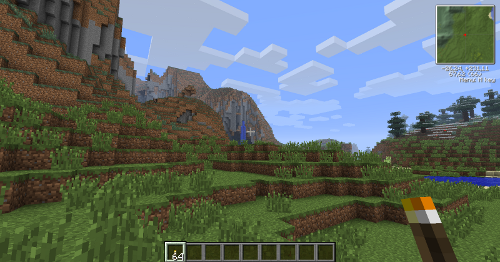
\includegraphics[width=9cm,   height=7cm]{Images/Terrain.png}
								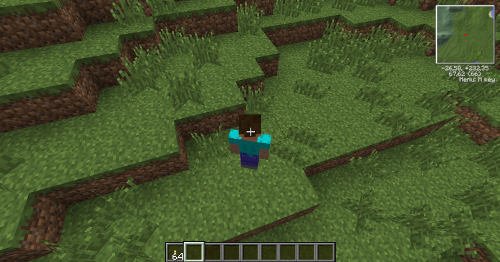
\includegraphics[width=8.5cm, height=7cm]{Images/Terrain2.png}
								\begin{center}\it This images are from the game Minecraft\end{center}
							\end{figure}
								
								This character will have the ability to break those cubes or add others. But what makes it an \ac{RTS} is the fact that he will be able to control other units, send them to combat and join them. Of course, for it to be an \ac{RTS} he will have to face opponents that we be controlled by the AI or you could play against other players.\\
								
								The character will also have the option to be able to add buildings that will be constructed by workers. Those will be the buildings that usually spawns units.\newline
								As you have already guessed the goal will be to eXplore, eXpand, eXploit, and eXterminate. But you will also have a scenario if you wish to play one.\newline
								Finally, you will also be able to face other players intense strategic battles.
						\section{Background} 
							This is year 2432, humans have spread throughout the universe. But criminality rates have been exploding for a decade. Thus a decision has been made to create jail planets. Therefore, any human proven guilty of any crime shall be exiled to those planets.\\
							
							During these past years, justice was harsh and you were one of the many sent to those planets that were innocent.\\

							However the stellar ship that was supposed to drop you on the planet was hit by meteorites. Still, you survived unharmed using the escape pods.  The planet where you were sent has a little particularity : it is composed of flying islands. You are now on one of the many islands which compose this planet.\\

							\begin{figure}[h]
								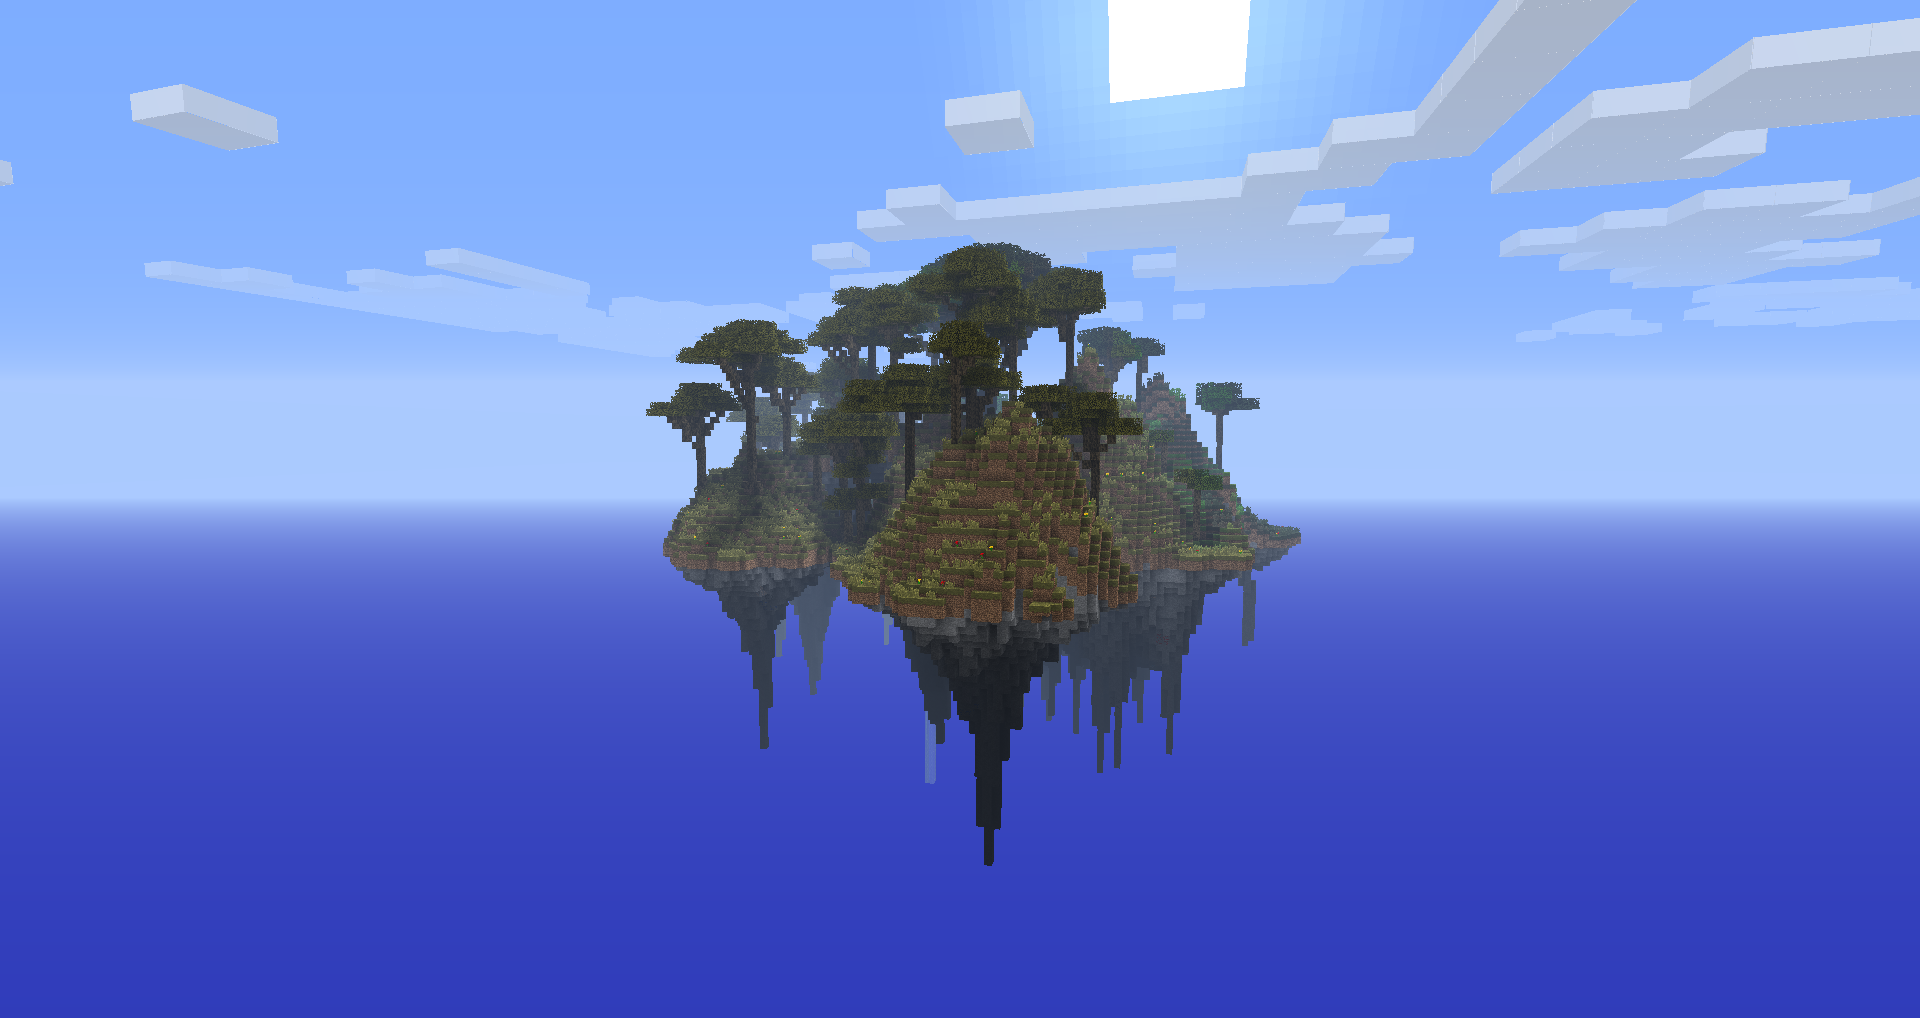
\includegraphics[width=16cm]{Images/FlyingIslands.png}
								\begin{center}\it This image is from the game Minecraft\end{center}
							\end{figure}

				\chapter{\textcolor{blue}{Goals \& interest}}
						\section{Learning new languages}
								Since half of the group are inexperienced programmers, one of the major goal of the project will be to learn about \textbf{clean} computer programming.\\
								
								Of course it will not be limited to C\#, because of the fact that we are working with \ac{OO} and learning clean computer programming and to ensure that everybody can understand the code, we will be using \ac{UML}.\newline
																							
								Also learning about clean computer programming means that we will be using some \ac{OO} well known principles such as inheritance and abstract class.
							  
						\section{Learning about web}
							  		Since \ac{PHP} is a easy to use and well known language, we will be using it. But, we will use the Symfony2 framework with Doctrine (which is an \ac{ORM} that permits to represent data as objects).\newline 
							  		As for Symfony, it is a \ac{PHP} Web Development Framework. Thus it provides generic functionality and "helps" you writing clean code. \newline
What clean code means is the fact that symfony\textquoteright s own architecture helps organizing our code.\\
							  		
							  		The power of symfony lies in the \ac{MVC} organization. Indeed Symfony2 is developed in an architecture that separates the representation of information from the user\textquoteright s interaction with it.\newline
							  		 Thus when the user will try to access to a website URL, this URL will be submitted to the router, which will then call the right PHP function. After processing the data relative to its purpose, this function will then send variables to a TWIG page which will then be displayed.
							  		 
						\section{Learning about 3D}
								As you might have already understood, we are using \ac{Mogre} which is a scene-oriented, real-time, flexible 3D rendering engine 3D library.\newline
								The class library abstracts the details of using the underlying system libraries like Direct3D and OpenGL and provides an interface based on world objects and other high level classes.\\
								
								Thus, the user can choose between Direct3D and OpenGL without us having to rewrite the entire code for each libraries. As its name states, \ac{OGRE} is "just" a rendering engine. As such, its main purpose is to provide a general solution for graphics rendering. Though it also comes with other facilities (vector and matrix classes, memory handling, etc.), they are considered supplemental. It is not an all-in-one solution in terms of game development or simulation as it does not provide audio or physics support, for instance.\\
								
								You should also know that having an experience with 3D is generally far more interesting than having an experience with 2D. Thus we decided to do some 3D.
								
								
				\chapter{\textcolor{blue}{Behind the scene}}
				
     					\section{Language \& Game design pattern}
     						Our project will be coded in \textbf{C\#} .NET 4.0 mainly because of the \ac{OO} paradigm and also for the large choice there is about 3D engine and libraries. The \ac{OO} let us use the \textbf{game state} pattern in order to structure the code. Basically, we consider our game as a stack of different states. Here is an example of a game state:
						\begin{figure}[h]
							
							\centering
							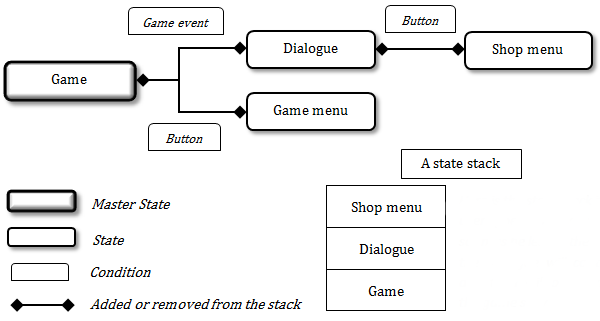
\includegraphics[height=242px]{Images/GameStateDesign.png}
							\it \\ There is always a master state at the beginning of the stack. Then other states may be added or removed; only the state at the top of the stack is updated and drawn. Depending on some condition as an input entry or a game event, each state can call any other states via a state manager.
						\end{figure}

						\begin{textblock}{0.128}(0.719, 0.625)
							\noindent \it 	Here is the state stack if the user goes to a shop. As soon as he leaves the shop, the dialogue will continue and then will only remain the game state.
						\end{textblock}
     						
     						This pattern is advised for \ac{RTS} games, among others. As we are working in a group, it is important to keep homogeneity throughout the program. Besides, a well-structured code will be easier to understand and to edit.
						
						\section{3D Engine \& Library}
						
						The 3D engine we will use is \textbf{\ac{Mogre}}. Initially, this is an \ac{API} coded in C++ called OGRE; Mogre is an advanced .NET 2.0 wrapper for OGRE. We have chosen this \ac{API} since it is known as an effective, handy and well-documented 3D engine in C\#.\\			
						Our \ac{GUI} will be implemented with the library \textbf{\ac{MyGUI}}. It is very flexible since all parameters are settable directly in the XML\textquoteright s files.\\	
						Since our 3D engine does not handle sound we have to use an audio library. We will use \textbf{NAudio} - an open source .NET library - because of its simplicity and completeness.
						
						\section{Softwares}
						
							Our \ac{IDE} will be \textbf{Visual Studio 2010 Ultimate}. We will also need \textbf{Blender} so that we can create our own meshes and then use them for our game with the script Blender2Ogre. Basically, all of our 3D objects will be created with Blender except for the terrain\textquoteright s cubes which are generated directly in the source code.
						The 3D engine we will use is \textbf{\ac{Mogre}}. Initially, this is an \ac{API} coded in C++ called OGRE; Mogre is an advanced .NET 2.0 wrapper for Ogre. We have chosen this \ac{API} since it is known as an effective, handy and well-documented 3D engine in C\#.\\		
							
							There are two key points in our projects which will have to be implemented using some well-known algorithms:
							\begin{itemize}
									\item \textbf{Terrain generation}. We want our land to be generated pseudo-randomly in order to create realistic islands - apart the fact that they are suspended in the sky. We want our islands to have mountains, jungles and rivers but we will definitely not build them ourselves. What we need to implement is the algorithm of \textbf{Perlin noise} in 3 dimensions. The idea for one dimension is to generate a list of random points, then to create a function which goes through these points. We repeat this step many times with an amplitude between the points getting smaller and smaller and then we add all the functions obtained. The concept is the same in 3 dimensions.\\

									\item \textbf{Pathfinding}. This is part of the \ac{AI} for the \ac{NPC}. The goal is to find the shortest way from a point A to a point B. A common solution for this problem is the \textbf{A*} (A star) algorithm. Basically, it tests all possibilities of path and then remembers the path which is getting closer to the arrival. This method is efficient and quick as long as there is no intricate labyrinth that is why we think A* is adapted for our project.
							\end{itemize}
				\chapter{\textcolor{blue}{Planning}}
					We decided to split the work into functional tasks. Thus we first decided to ask each member\textquoteright s preference. After asking them about it, we decided to divide the game as the following table : 
					\begin{center}
						~~~~~~~~~~~~~~\begin{tabular}{|c|c|c|c|c|}
							\hline
								%\centering
								%{First oral}  & Renaud & Aenora & Erwan & Romain \\
									%\textbf{ First oral & Renaud & Aenora & Erwan & Romain}
								~~~~~~~~~~~~~~ \textbf{First oral} ~~~~~~~~~~~~~~  & \textbf{Renaud} & \textbf{Aenora} & \textbf{Erwan} & \textbf{Romain} \\
							\hline 
						 		Terrain generation & + & + &  &  \\
							\hline
						 		Player &  &  & + & +  \\
							\hline
						 		Sky &  &  & + & +  \\
							\hline
						 		Web Site & + & + & + & +  \\
							\hline
								 Menu &  & + &  & +  \\
							\hline
						\end{tabular}
\newline

						~~~~~~~~~~~~~~\begin{tabular}{|c|c|c|c|c|}
							\hline
								\textbf{Second oral} & \textbf{Renaud} & \textbf{Aenora} & \textbf{Erwan} & \textbf{Romain} \\
							\hline
								 \ac{NPC} with simple \ac{AI} & + &  &  & + \\
							\hline
								 Mouse actions &  &  & + & + \\
							\hline
								 Advanced menu &  & + &  & + \\
							\hline
								 Advanced terrain generation & + & + &  &  \\
							\hline
				 				Buildings &  &  & + & + \\
							\hline
						\end{tabular}
\newline

						~~~~~~~~~~~~~~\begin{tabular}{|c|c|c|c|c|}
							\hline
								~~~~~~~~~~~~~~ \textbf{Third oral} ~~~~~~~~~~~~~ & \textbf{Renaud} & \textbf{Aenora} & \textbf{Erwan} & \textbf{Romain} \\
							\hline
 								\ac{RTS} &  & + &  & + \\
							\hline
 								\ac{AI} & + &  & + &  \\
							\hline
 								Save & + & + &  &  \\
							\hline
						\end{tabular}
\newline

						~~~\begin{tabular}{|c|c|c|c|c|}
							\hline
								~~~~~~~~~~~~~ \textbf{Fourth oral} ~~~~~~~~~~~~  & \textbf{Renaud} & \textbf{Aenora} & \textbf{Erwan} & \textbf{Romain} \\
							\hline
 								Multiplayer &  &  & + & + \\
							\hline
								 Map \& story editor & + & + &  &  \\
							\hline
								 Story & + & + & + & + \\
							\hline
						\end{tabular}
\end{center}



				\chapter{\textcolor{blue}{Conclusion}}
					We hope that this project will help us in multiple domains of computer science such as 3D, \ac{OO}, web, \dots \\
					Also we are glad to sail for this great adventure that is realizing a 3D game. \\

					We acknowledge the difficulty of developing a 3D game but we are still motivated. Besides, we know that there will be "rush" periods. Still we will try our best to reduce those periods.\\
					We are confident that our objectives will be achieved for the fourth oral presentation.
\\ ~\\ ~\\ ~

					 

					


				\begin{center}
					
\includegraphics[width = 16cm]{Images/Islands_Title.png}
				\end{center}     	     		
\end{document}